% !TeX root = ../DistributedConsensus.tex
% !TeX spellcheck = en_GB
\chapter{Validation of Histories}\label{chap:validation}
	This chapter defines how histories from events on malicious processes are observed and possibly identified.
	
	\newpar We introduce malicious processes in distributed DCR graphs. The implementation allows multiple events to be hosted by a single process, but in this chapter it is assumed that any process only hosts a single event. Malicious processes corrupts data in many ways and therefore it is desired to have a mechanism which can observe, and if possible identify these corruptions and the processes which created them in a predictable way. 
    
    \newpar As mentioned in \autoref{def:validhistory} the valid history has the following properties:
    
    \begin{enumerate}
    	\item Actions in the history are not invented, changed or removed.
    	\item The rules of the workflow are followed.
    	\item The history abides to serial equivalence.
    	\item The history is in a strict partial order.
    \end{enumerate}
	
	\noindent Cheating is the act of creating histories which violates at least one of these properties. This leads us to two different kinds of cheating:
	
	\begin{definition}
		\textbf{Inconsistent cheating} violates property 1, and at least one of 2, 3, and 4.
		\label{def:inconsistentcheating}
	\end{definition}
	
	\begin{definition}
		\textbf{Consistent cheating} violates property 1, but not 2, 3, and 4.
		\label{def:consistentcheating}
	\end{definition}
	
	\noindent Definition \ref{def:inconsistentcheating} defines that inconsistent cheating is the act of creating a history which could not have happened, according to the rules of the workflow, serial equivalence or strict partial ordering of actions. Definition \ref{def:consistentcheating} defines that consistent cheating is the act of creating a history which could have happened, but did not.
	
	\newpar A malicious process is a process which participates in consistent or inconsistent cheating.
	
	\section{Inconsistent Cheating}
	To examine inconsistent cheating in depth, we must explore cheating where each of the properties 2, 3, and 4 are violated. We will see that either property violation can be identified separately.
		
	\subsection{DCR Rules}
	A given local history must abide to the rules of the workflow it has been created from. 
	In order to validate a local history against these rules, the events, their relations and the initial state of the workflow must be known. The following sections each describe an assertion that can be made in order to guarantee that the history has followed the rules of the workflow.\todo{Revise the last sentence}
	
	\newpar As seen in \autoref{chap:representing-a-history} actions are based on the effects that happen when an event executes. Actions match the relations of a workflow, if the event ID, counterpart ID and action type correspond to the start node, end node, and type of the relation in the DCR graph. We will use this notion to explain the DCR rules that a history must follow.
	
	\begin{ruledef}
		\textbf{Only specified relations}: The local history of an event must only contain actions of corresponding relations in the workflow.
		\label{rule:validrelations}
	\end{ruledef}
	
	\noindent An example of a DCR graph and the local histories of the events are shown in \autoref{fig:validation:only-specified-relations}. All events, $A$, $B$, and $C$, contain relations that are not specified in the workflow.
	
	\begin{figure}[H]
		\centering
		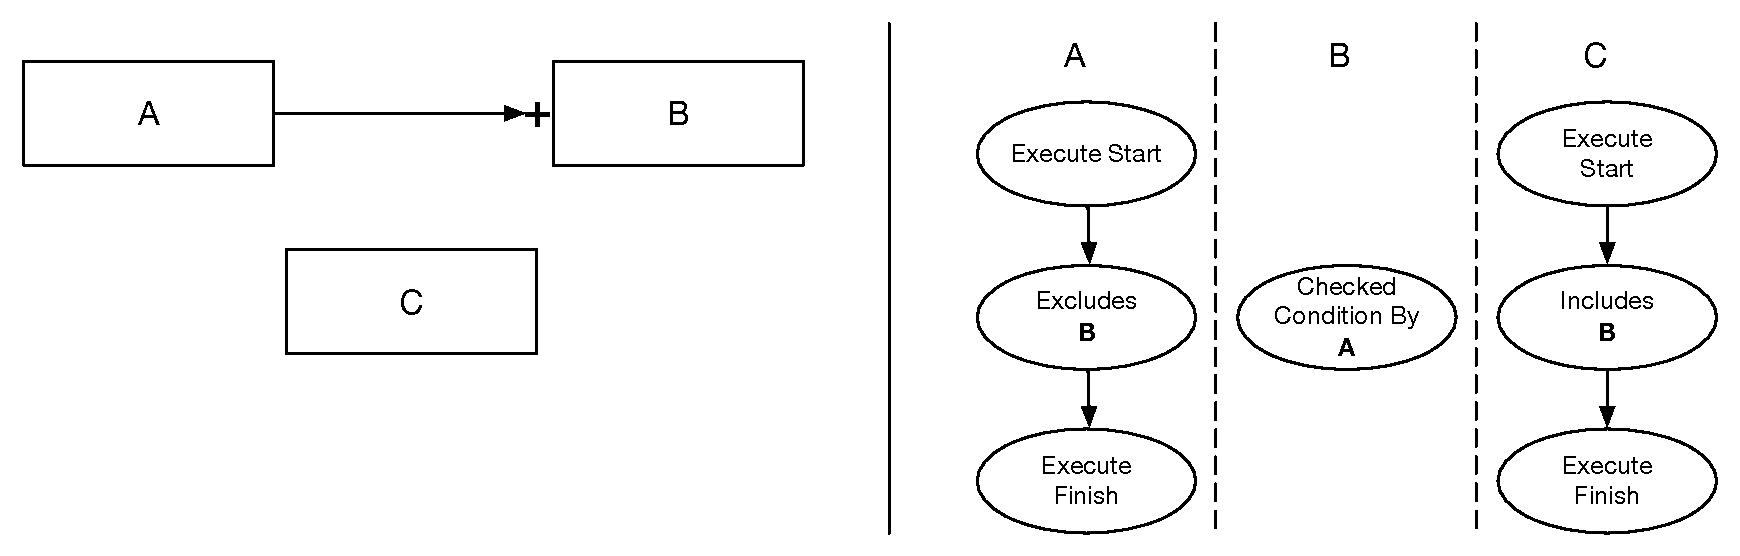
\includegraphics[width=\textwidth]{5validation/images/only-specified-relations.pdf}
		\caption{A DCR graph and three examples of local histories violating \autoref{rule:validrelations}.}
		\label{fig:validation:only-specified-relations}
	\end{figure}
	
	\noindent It can be validated that local histories adhere to \autoref{rule:validrelations} by examining every action, and for each outgoing and incoming action, the event, its counterpart, and action type must be present in the rules of the workflow.
	
	\begin{ruledef}
		\textbf{Only complete executions}: A given event, $E$, must have actions for each of its outgoing relations when executing. Each of the counterparts of these actions must have a corresponding action in their history after $E$ has executed. For any execution there must be exactly one action of type \textup{Execute start} happening before a single action of type \textup{Execute finish}.
		\label{rule:completeexecutions}
	\end{ruledef}

	\begin{figure}[H]
		\centering
		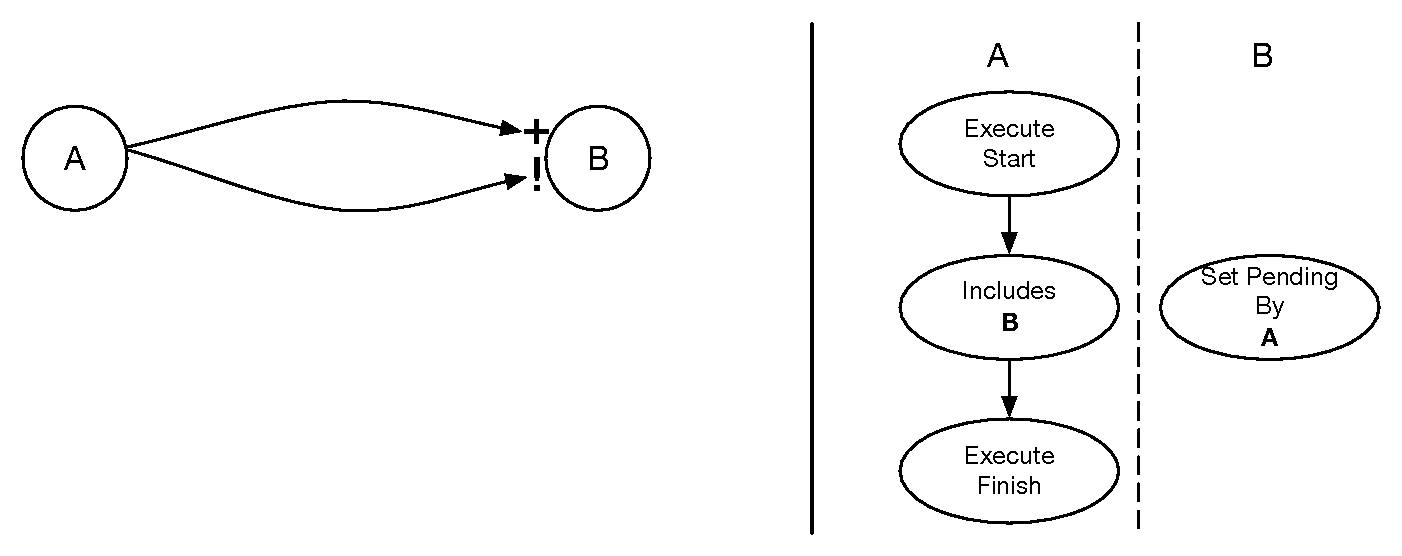
\includegraphics[width=\textwidth]{5validation/images/only-complete-executions.pdf}
		\caption{A DCR graph and two examples of local histories violating \autoref{rule:completeexecutions}.}
		\label{fig:validation:only-complete-executions}
	\end{figure}

	\noindent In \autoref{fig:validation:only-complete-executions} event $A$ does not contain an outgoing action of type \textit{Sets pending} and event $B$ does not contain an incoming action of type \textit{Included by}.

	\newpar In order to validate \autoref{rule:completeexecutions} for outgoing relations the following approach is taken: When an action of type \textit{Execute start} is encountered in the local history, a set of required actions for the execution is created from the rules of the workflow.
	
	For example, if event $A$ includes event $B$ and excludes itself, this set must contain an outgoing action corresponding to the inclusion of $B$, and two actions, one outgoing and one incoming, corresponding to the exclusion of event $A$ itself.
	
	Each consecutive action in the history, must be one of the actions in the set. The action is then removed from the set. When the set is empty, the next action in the history must have type \textit{Execute finish}.
	
	\newpar In order to validate \autoref{rule:completeexecutions} for incoming relations where the counterpart is not the event iself the following approach is taken: When an incoming action from an event $A$ is found, all actions corresponding to the remaining rules that specify that $A$ has a relation to the current event, is added. While the set is not empty, the consecutive actions in the history must exist in the set. An action is removed from the set when it is encountered.

	\begin{ruledef}
		\textbf{Executions only in Valid States}: The history of an event must only contain executions when the event is executable. This implies that the entirety of the history must match a run of the DCR graph it represents.
		\label{rule:executionvalidstate}
	\end{ruledef}
	
	\noindent Checking for this kind of inconsistency is nontrivial. A method of doing so is described in \autoref{sec:historyindcr:simulation}.
	
	To argue that rules \ref{rule:validrelations} through \ref{rule:executionvalidstate} covers the DCR rules, the definition of DCR graphs is examined. In \autoref{sec:background:dcrgraphs} the definition of a DCR graph is described. From the definition it is possible to make a set of all relations where each element is a triple of two events and the type of the relation. Because this set is finite, \autoref{rule:validrelations} makes sure that the actions can only represent the relations that exists in that set. Furthermore since the relations can be filtered by events it is possible to get the set of relations that happen in an execution. This is ensured by \autoref{rule:completeexecutions} which makes sure that every action that should happen, happens in an execution. The definition of DCR graphs also declares what the state of the workflow must be for an event to be executable and we will see in \autoref{sec:historyindcr:simulation} that this case is also covered. The definition of a DCR graph does not have any more requirements for the run of a workflow and therefore these rules must cover all kinds of cheating which contradicts the rules of the workflow.
	
	\subsection{Serial Equivalence Rules}
	A given execution must comply to the rules of serial equivalence. That includes the following:
	
	\begin{ruledef}
		\textbf{Only non-disrupted executions}: A given event, $E$ must not contain ingoing relations or execute starts when already executing. Furthermore if an execution is started, it must also finish. The exception to the rule of ingoing relations is when an event has a relation to itself in which case that incoming action is allowed.
		\label{rule:non-disruptedexecutions}
	\end{ruledef}
	
	\noindent Figure \ref{fig:validation:only-non-disrupted-executions} shows an example where an execution of event $A$ is interrupted by an incoming action from another event.
	
	\begin{figure}[H]
		\centering
		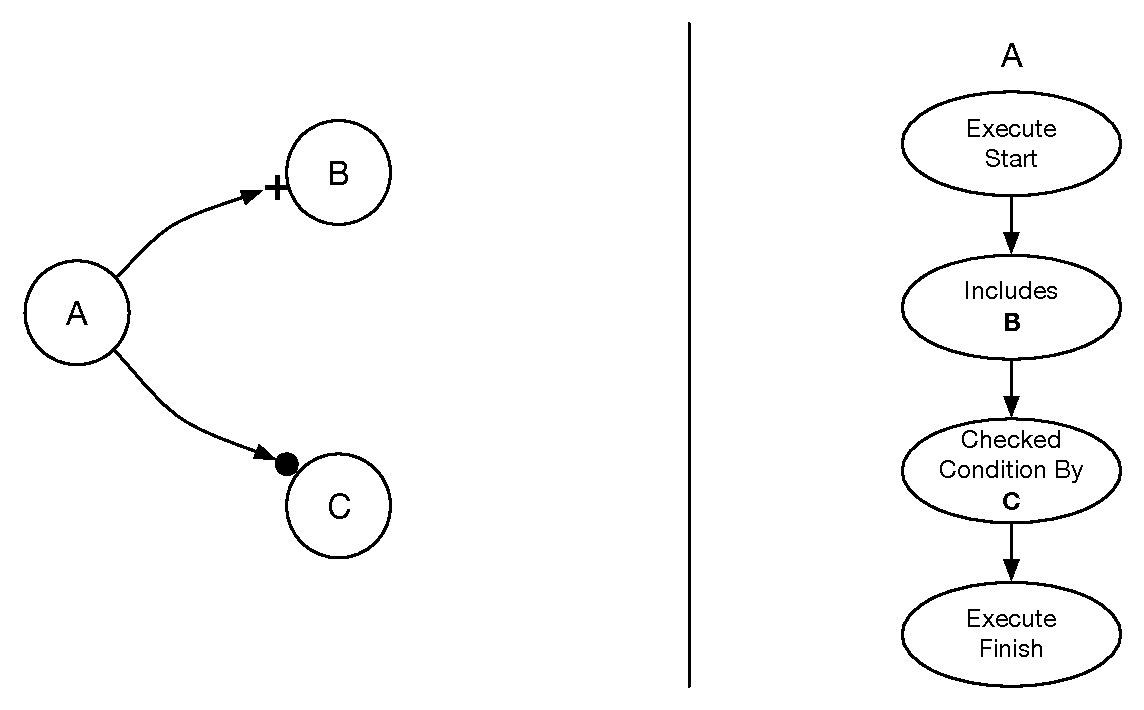
\includegraphics[width=.7\textwidth]{5validation/images/only-nondisrupted-executions.pdf}
		\caption{A DCR graph and an example of a history where \autoref{rule:non-disruptedexecutions} is violated}
		\label{fig:validation:only-non-disrupted-executions}
	\end{figure}
		
	\noindent The algorithm used to check \autoref{rule:completeexecutions} for outgoing relations is also used to check \autoref{rule:non-disruptedexecutions}.
	
	\begin{ruledef}
		\textbf{Wait for complete execution}: A given event, $A$ must be affected by all its ingoing relations from an event, $B$ when $B$ executes before anything else happens. The exception to the rule is when an event has a relation to itself in which case actions from the execution are allowed before the next incoming action happens. 
		\label{rule:wait-for-complete-execution}
	\end{ruledef}
	
	\noindent Figure \ref{fig:validation:wait-for-complete-execution} shows a situation where $B$ is included by $A$ but executes before the response relation from $A$ is present in the history.
	
	\begin{figure}[H]
		\centering
		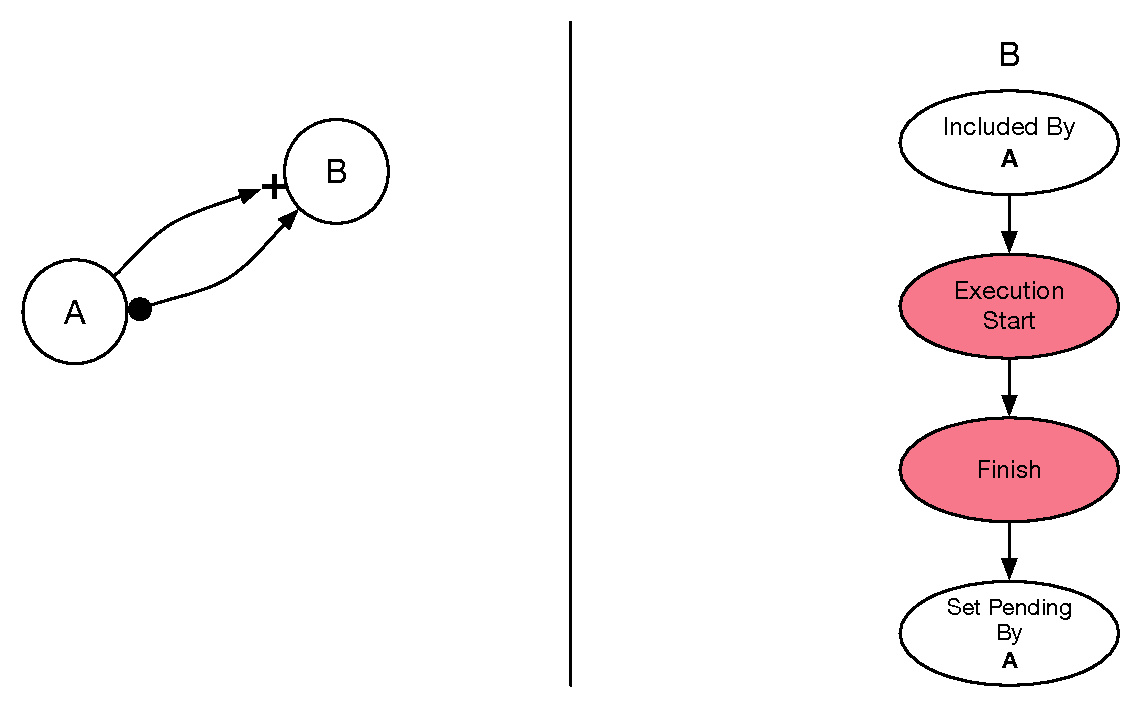
\includegraphics[width=.7\textwidth]{5validation/images/wait-for-complete-execution.pdf}
		\caption{A DCR graph and an example of a history where \autoref{rule:wait-for-complete-execution} is violated}
		\label{fig:validation:wait-for-complete-execution}
	\end{figure}
	
	\noindent The algorithm used to check \autoref{rule:completeexecutions} for incoming relations is also used to check \autoref{rule:non-disruptedexecutions}.
		
	\begin{ruledef}
		\textbf{Synchronous Message Exchanges}: If message exchanges happen synchronously outgoing or incoming actions must have counterpart timestamps higher than any counterpart timestamp of actions that happen before it.
		\label{rule:total-order-counterpart-timestamps}
	\end{ruledef}
	
	\noindent A validation of this kind of inconsistency can be done on each single event. Since each incoming and outgoing action must have a counterpart, it is possible to keep a mapping between counterparts and the last timestamp that counterpart had. Recall that the implementation requires that all correct processes only accept higher timestamps for a counterpart, than any timestamp seen from that counterpart before. \todo{Husk at skrive dette!} If a new timestamp for a counterpart is lower than the previous, then the event must be malicious.
	
	\begin{figure}[H]
		\centering
		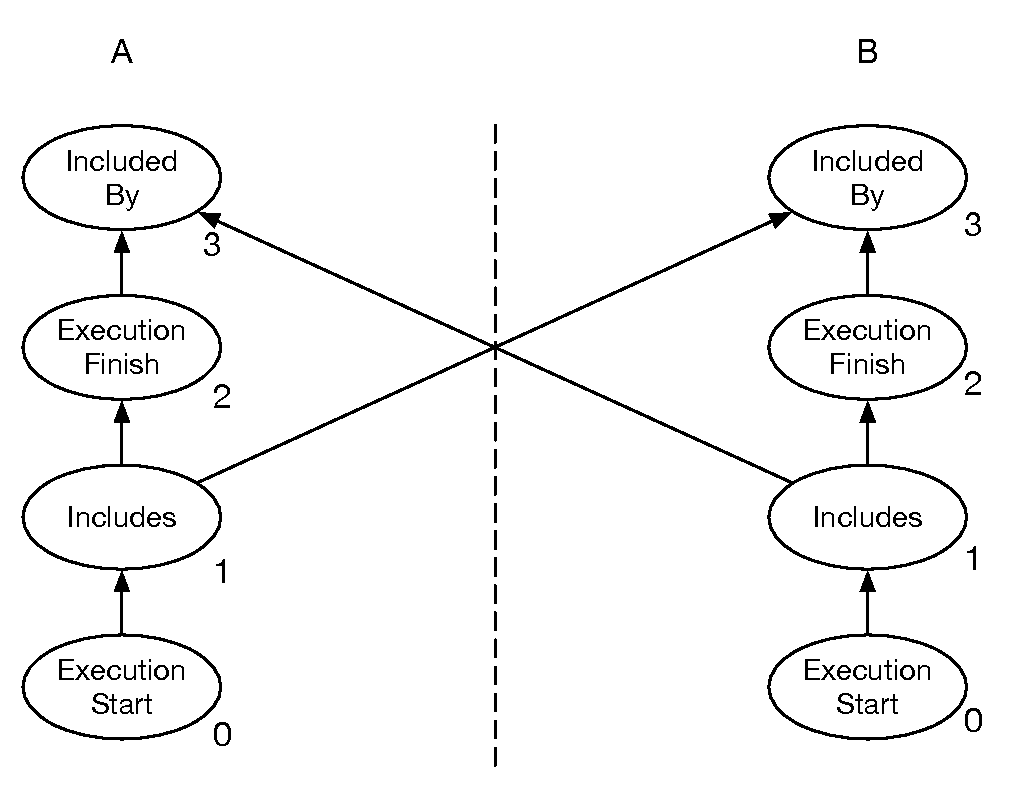
\includegraphics[width=.5\textwidth]{5validation/images/total-order-of-counterpart-timestamps-cycle.pdf}
		\caption{An example of two local histories violating \autoref{rule:total-order-counterpart-timestamps}.}
		\label{fig:validation:total-order-of-counterpart-timestamps}
	\end{figure}
	
	\newpar Figure \ref{fig:validation:total-order-of-counterpart-timestamps} shows a situation where the counterpart timestamps are not in order on neither event A nor B which violates \autoref{rule:total-order-counterpart-timestamps}. Because the implementation requires serial equivalent executions, and because message transfers happen synchronously such a violation will never happen on a correct process, as this would imply a pair of executions which happens before each other. Imagine the situation on the \autoref{fig:validation:total-order-of-counterpart-timestamps}, event A includes B and sets the counterpart timestamp to 3. Then it finishes its execution and gets included by B, but it receives a counterpart timestamp of 1. This must imply one of two things, either the timestamps on event B are out of order, or event B has been executing and accepting incoming actions simultaneously, creating a situation which is not serially equivalent. 
	
	\newpar To argue that rules \ref{rule:non-disruptedexecutions} through \ref{rule:total-order-counterpart-timestamps} cover the requirements of serial equivalence, recall that serial equivalence requires that any interleaving of transactions must create the same result, as if the transactions had happened in sequence. The implementation of a correct process in distributed DCR graphs must therefore only allow executions of events in a serially equivalent manner. As described in \autoref{sec:background:implementation} the provided implementation uses locking to achieve serial equivalence. Furthermore all message exchanges happen synchronously, that is the sending process receives confirmation that the message has been received, before continuing the execution. In the implementation, \todo{beskriv dette sammen med stedet der skal beskrive hvornår vi gemmer ting?}an action of type \textit{Execute start} is saved when a process has received all locks on events it affects during the execution of an event. Also an action of type \textit{Execution finish} is saved just before all locks are released. This means, for all correct processes, any group of actions representing an execution must be performed when all affected events are locked. Furthermore no actions from other executions must be present in between the actions of an execution. If this property is violated, this can be present in histories in the following three ways:
	
	\begin{itemize}
		\item An incoming action is inside an execution of another event. This is the case presented in \autoref{fig:validation:only-non-disrupted-executions} and can be found by applying \autoref{rule:non-disruptedexecutions}.
		\item Any action, not part of an execution $E$, is between at least two incoming actions part of execution $E$. This is the case presented in \autoref{fig:validation:wait-for-complete-execution} and can be found by applying \autoref{rule:wait-for-complete-execution}.
		\item In a local history an action of type \textit{Execute start} has a path to another action of type \textit{Execute start} in which no action of type \textit{Execute finish} exists. This case can be found by applying \autoref{rule:non-disruptedexecutions}.
	\end{itemize}
	
	Together these three ways of violating serial equivalence cover all cases of an event being affected while being locked. There is a case where two processes can participate in the creation of a history where each of the local histories are serially equivalent but when the actions of the executions are connected, serial equivalence is violated because message exchanging was not done synchronously. Figure \ref{fig:validation:synchronous-execution} illustrates a history and how it would look like if message confirmations were stored as part of synchronous message exchanges. This also explains why the situation in \autoref{fig:validation:total-order-of-counterpart-timestamps} is not valid because a cycle would be present if message confirmations were explicit as seen in \autoref{fig:validation:explicit-message-confirmations}. Because of this it can be concluded that both the execution of event $A$ and $B$, happens before each other. Serial equivalence requires that the interleaving is equivalent to the execution of one of the events first followed by the other, it can be concluded that this interleaving is not serially equivalent. This last form of serially equivalence violation is covered by \autoref{rule:total-order-counterpart-timestamps}.
	
	\begin{figure}[H]
		\centering
		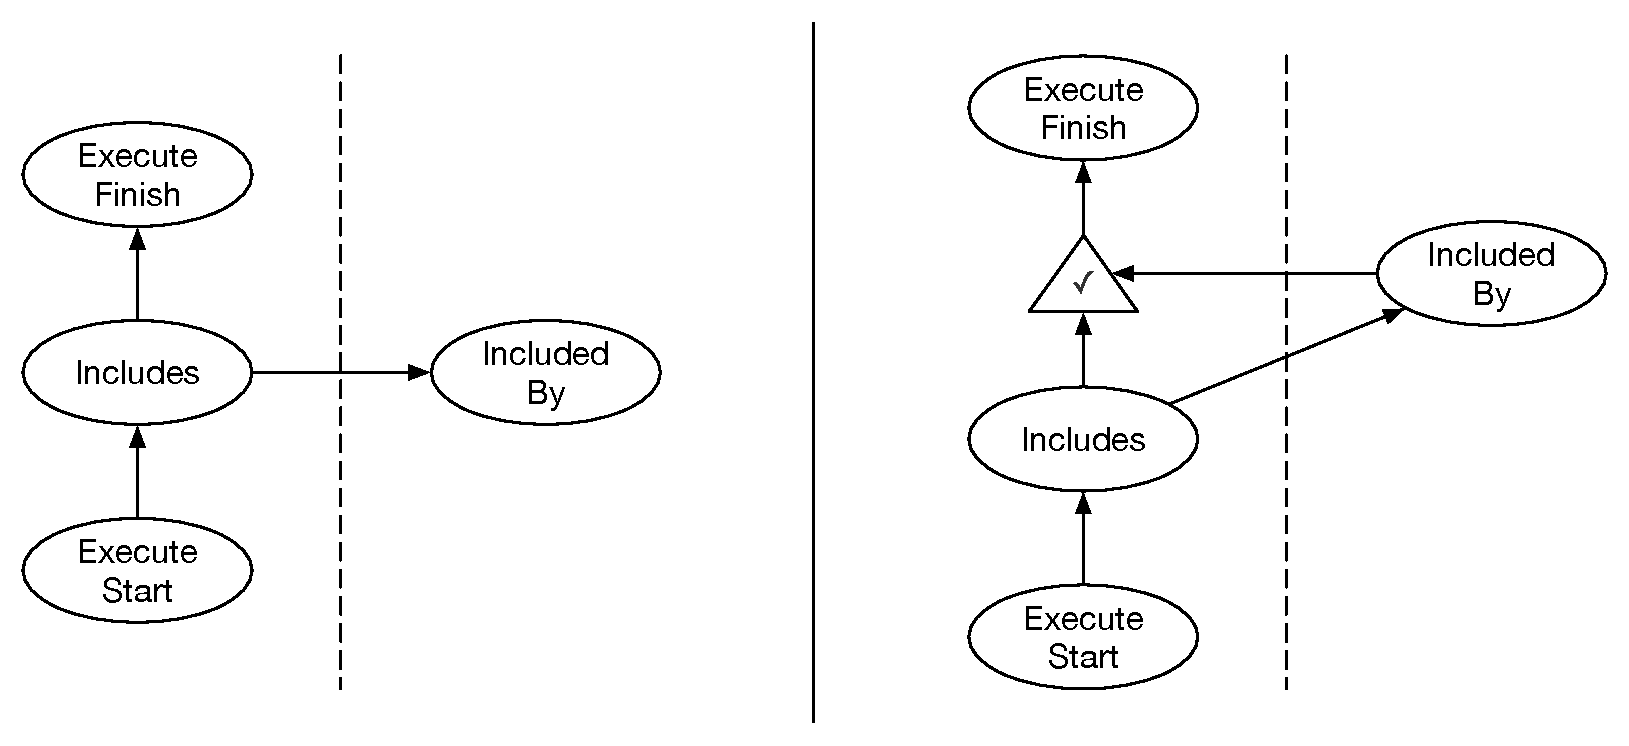
\includegraphics[width=0.8\textwidth]{5validation/images/synchronous-execution.pdf}
		\caption{An illustration of how message exchanges correspond to synchronous communication.}
		\label{fig:validation:synchronous-execution}
	\end{figure}
	
	\begin{figure}[H]
		\centering
		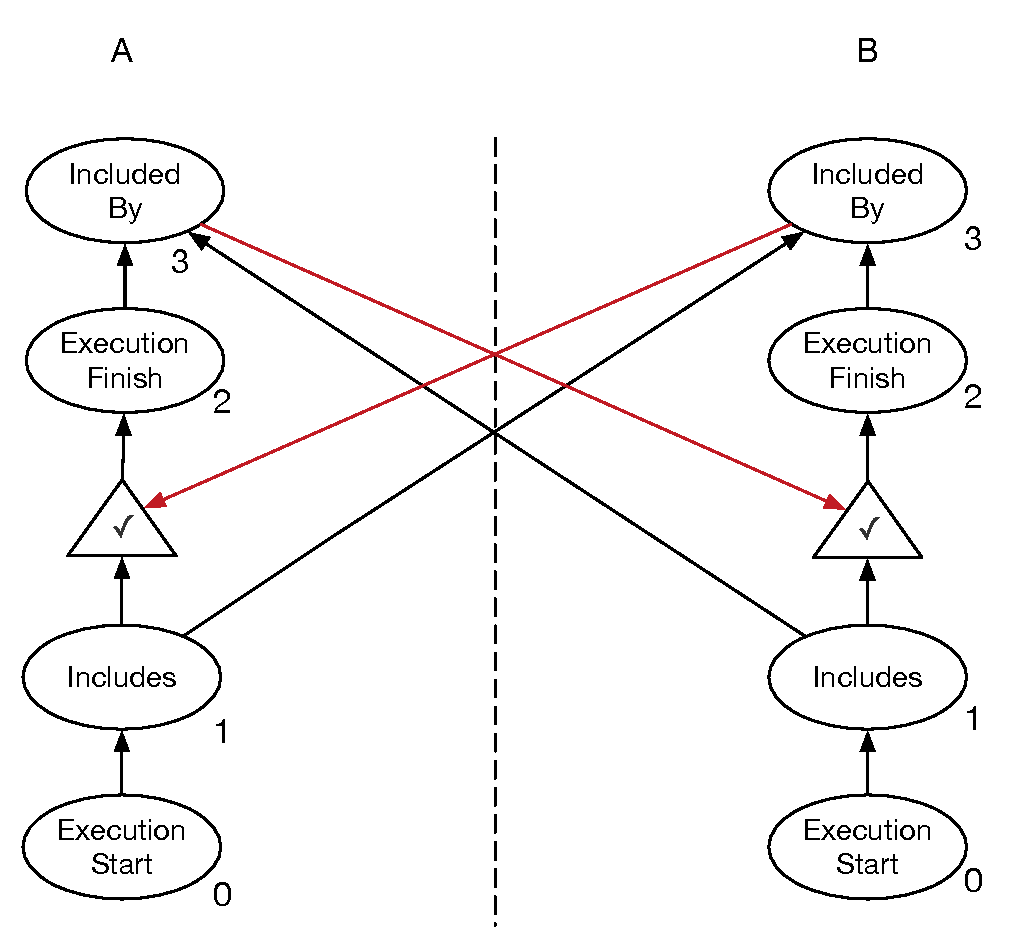
\includegraphics[height=0.3\textheight]{5validation/images/total-order-of-counterpart-timestamps-cycle-confirmation.pdf}
		\caption{An illustration of cycles shown when message confirmations are made explicit.}
		\label{fig:validation:explicit-message-confirmations}
	\end{figure}
	
	\subsection{Lamport's Logical Clocks}
	A given history must conform to the rules of Lamport's logical clocks. That includes the following:
	
	\begin{ruledef}
		\textbf{Total Order of Timestamps}: Every action in the local history of an event must have a timestamp less than the timestamp of any action it happens before.
		\label{rule:total-order-timestamps}
	\end{ruledef}
	
	\noindent This kind of inconsistency can be checked by examining each action on a single event. If the timestamps are not increasing for each edge in the graph then the event must be cheating.
	
	\begin{ruledef}
		\textbf{Message Exchange Timestamp Order}: For every pair of actions that represent a message exchange, the timestamp of the outgoing action must be less than the timestamp of the incoming action.
		\label{rule:message-exchange-timestamp-order}
	\end{ruledef}
	
	\noindent A validation of this kind of inconsistency can be done on the history of each event. If the counterpart timestamps of the outgoing actions are not larger than the timestamps then the event is malicious. For incoming actions the counterpart timestamp must be less than the timestamp.
	
	\newpar Because histories are represented as directed acyclic graphs, cycles must not exist. Rule \ref{rule:total-order-timestamps} and \ref{rule:message-exchange-timestamp-order} makes it possible to observe cycles and identify the local histories from where the cycles originate.
	
	Together, these rules make sure that no cycles can exist. If an action happens before another action with a lower timestamp, at least one of rules \ref{rule:total-order-timestamps} and \ref{rule:message-exchange-timestamp-order} have been violated. Examples of violations of rules \ref{rule:total-order-timestamps} and \ref{rule:message-exchange-timestamp-order} are shown in figures \ref{fig:validation:message-exchange-timestamp-order-cycle} and \ref{fig:validation:message-exchange-timestamp-order-cycle}.
	
    \begin{figure}[H]
		\centering
    	\begin{minipage}{.45\textwidth}
			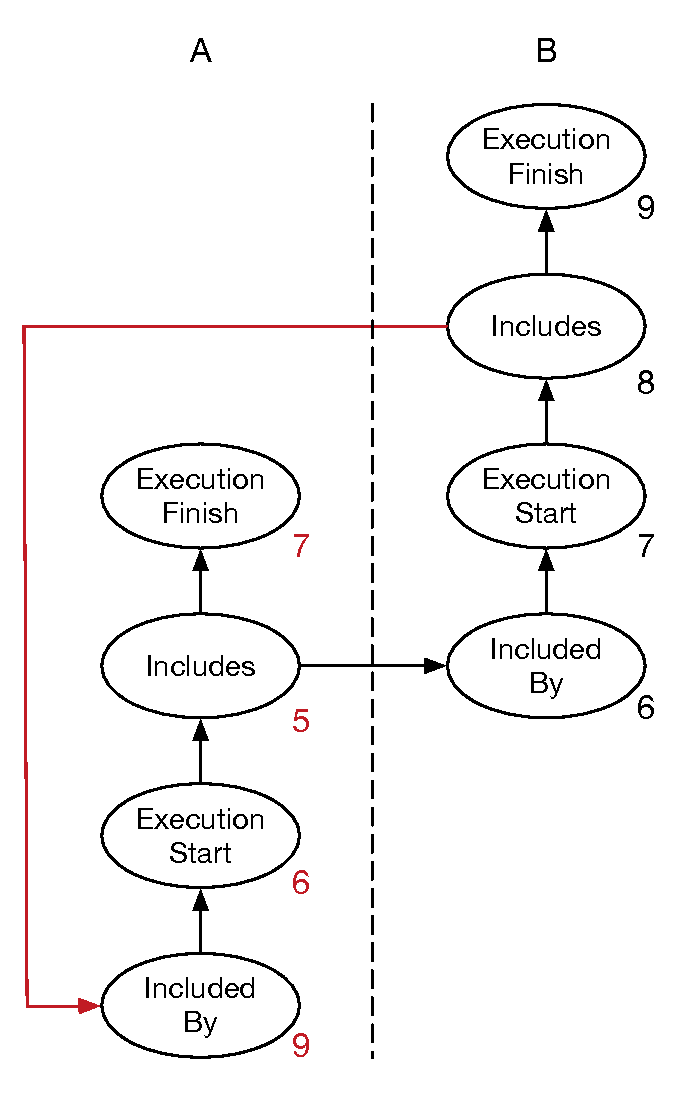
\includegraphics[width=.89\textwidth]{5validation/images/total-order-of-timestamps-cycle.pdf}
			\caption{An example of two histories forming a cycle by violation of \autoref{rule:total-order-timestamps}.}
			\label{fig:validation:total-order-of-timestamps-cycle}
    	\end{minipage}
		\hfill
		\begin{minipage}{.45\textwidth}
	    	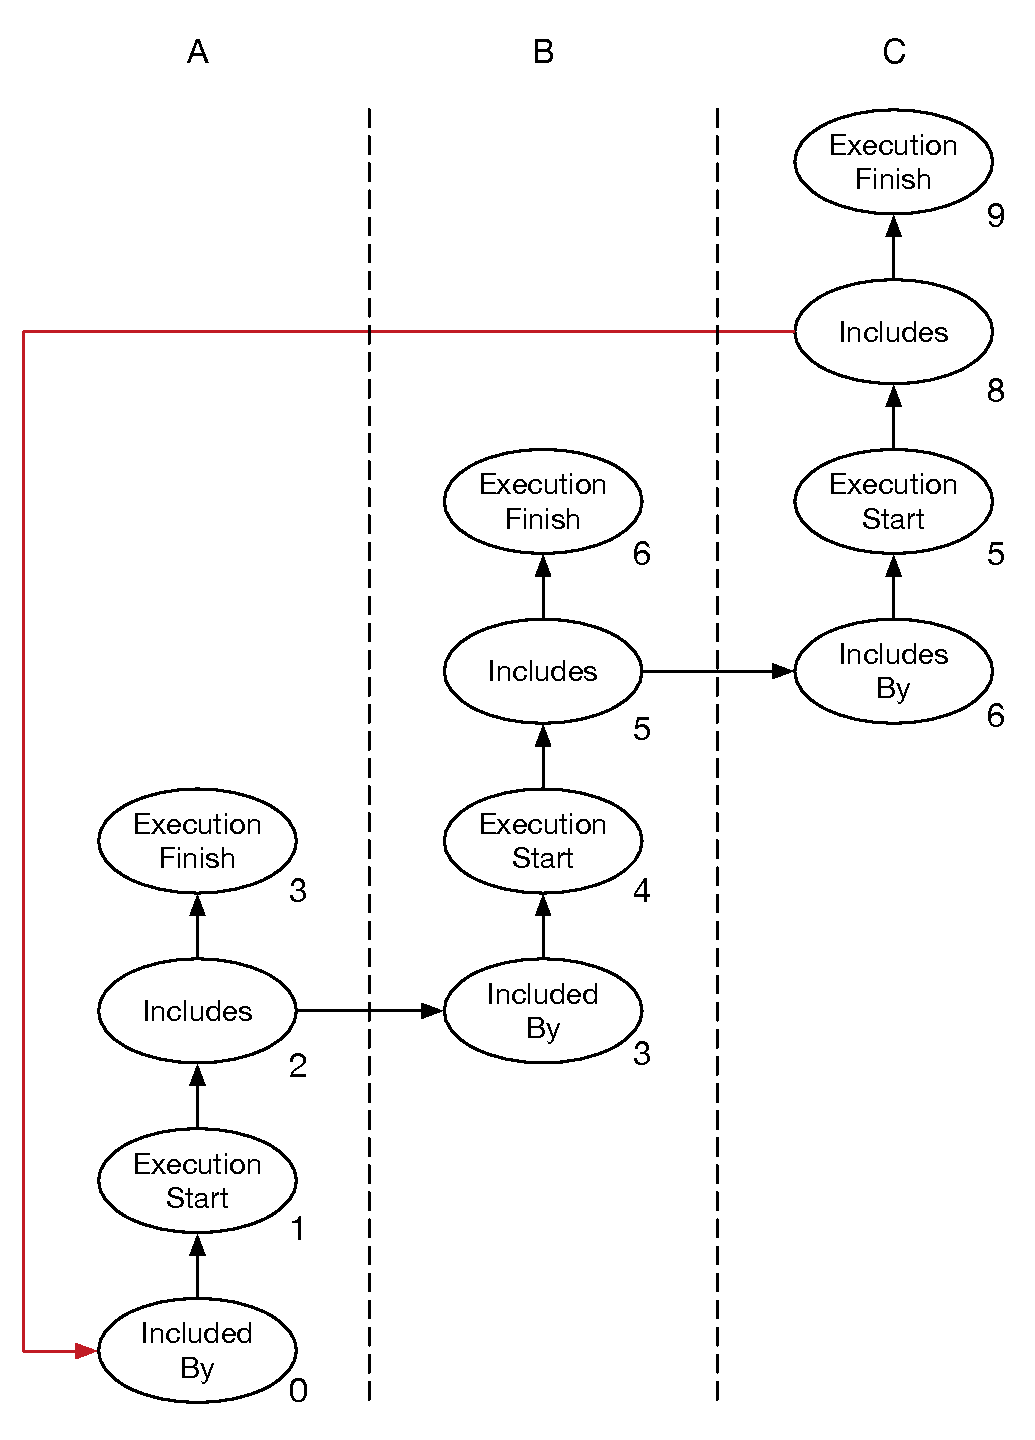
\includegraphics[width=\textwidth]{5validation/images/message-exchange-timestamp-order-cycle.pdf}
	    	\caption{An example of three histories forming a cycle by violation of \autoref{rule:message-exchange-timestamp-order}.}
	    	\label{fig:validation:message-exchange-timestamp-order-cycle}
		\end{minipage}
	\end{figure}
	
	\noindent On \autoref{fig:validation:total-order-of-timestamps-cycle} a cycle is created when event $A$ changes the order of its actions, violating \autoref{rule:total-order-timestamps} while still keeping the timestamps of message exchanges in an increasing order.
	
	\newpar On \autoref{fig:validation:message-exchange-timestamp-order-cycle} a cycle is created when timestamps of message exchanges are not kept in an increasing order, violating \autoref{rule:message-exchange-timestamp-order}. The timestamps of actions in the local histories are in increasing order which means that \autoref{rule:total-order-timestamps} is not violated.
	
	\newpar To argue that rules \ref{rule:total-order-timestamps} and \ref{rule:message-exchange-timestamp-order} cover the requirements of Lamport's logical clocks, recall that Lamport states that the timestamp of a given action on a given process must be lower than any action it happens before. This is covered by \autoref{rule:total-order-timestamps}.
	
	Lamport also states that for any message exchange between two processes, the local timestamp of the process receiving the event, must be set to a higher timestamp than that of the sending process. This is covered by \autoref{rule:message-exchange-timestamp-order}. Together these two rules cover the requirements of Lamports logical clocks.
	
	\section{Consistent Cheating}
	Until now we have examined inconsistent cheating, but malicious processes are also able to cheat consistently. Recall that consistent cheating is the act of creating histories which \textit{could} have happened but did not. In this section \textit{original} actions and timestamps are actions and timestamps that did happen in the execution of the workflow. 

	\newpar Consistent cheating is present if one of the following rules are violated:

	\begin{ruledef}
		\textbf{Agreement on original timestamps}: Two events must agree on the original timestamps of their actions corresponding to their relations to each other.
		\label{rule:agreement-on-original-timestamps}
	\end{ruledef}
	
	\noindent When actions are matched together to form happens before relations between the histories of two events, the timestamps and counterpart timestamps are used to uniquely identify a pair of matching actions. If however it is not possible to match actions because timestamps are mismatched, then at least one of the histories must have been changed. 
	
	\begin{figure}[H]
		\centering
		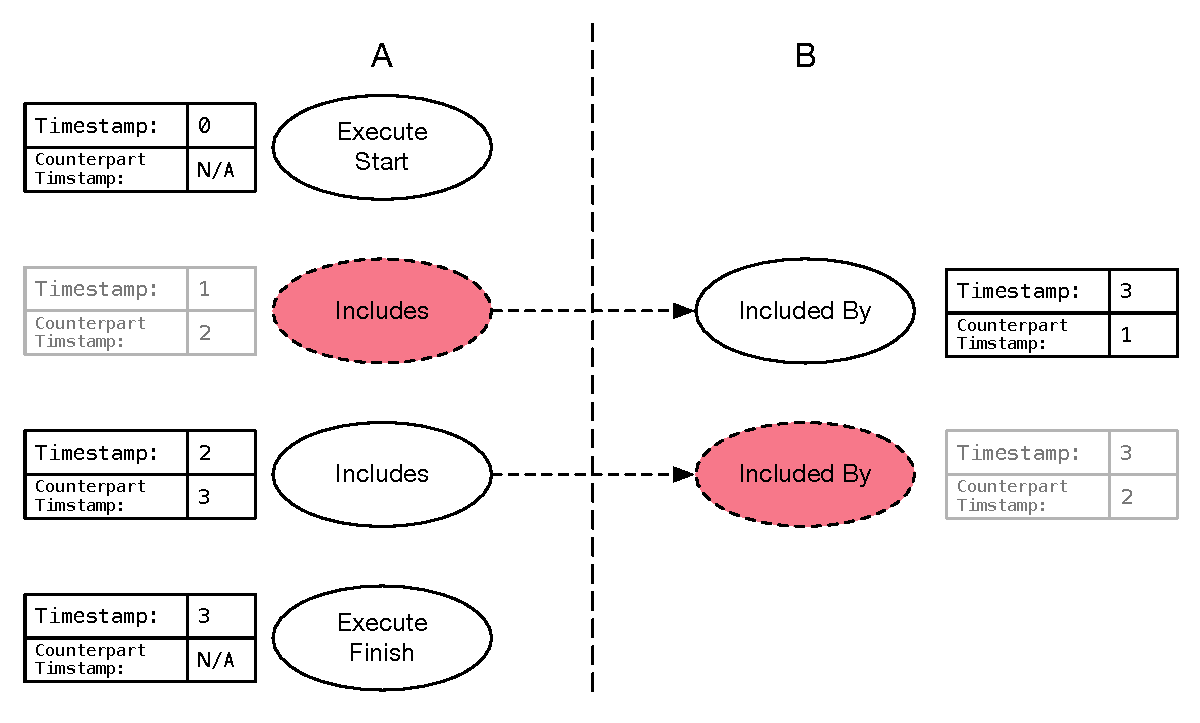
\includegraphics[width=0.7\textwidth]{5validation/images/agreement-on-original-timestamps.pdf}
		\caption{An example of two local histories with no inconsistent cheating, not agreeing on the timestamps thereby violating \autoref{rule:agreement-on-original-timestamps}. Dashed actions marked with a red colour denote the actions which are not present but are expected by the counterpart.}
		\label{fig:agreement-on-original-timestamps}
	\end{figure}
	
	An example of two events not having matching actions in their histories because of the timestamps can be seen on \autoref{fig:agreement-on-original-timestamps}. Notice that it is not possible to distinguish the two include actions from each other, and that is therefore not possible to identify which of the two histories are invalid.
	
	\newpar To validate for this kind of cheating, pairs of local histories where a relation exists between them are examined. Each ingoing action is matched with outgoing actions and if it is not possible to find a match, one of the processes hosting the events must be malicious. Since the original timestamps are unknown, it is not possible to distinguish an original timestamp from an unoriginal one, and therefore two events can agree on unoriginal timestamps without failing this validation.
	
	\begin{ruledef}
		\textbf{Agreement on the original amount of executions}: If an event A has a relation to an event B then the two events must agree on the number of executions of A in their histories.%
		\label{rule:agreement-on-the-original-amount-of-executions}
	\end{ruledef}
	
	\noindent To check for this kind of cheating the local histories of each pair of events which are part of a relation are examined. If event $A$ and event $B$ are examined, then the amount of every outgoing action from $A$ to $B$ must match the amount of incoming actions on $B$ from $A$. If the amount does not match then one of the processes hosting the events must be malicious.
	
	\newpar On \autoref{fig:agreement-on-the-original-amount-of-executions-1} an example of violation of \autoref{rule:agreement-on-the-original-amount-of-executions} is shown. In the shown histories, event A states that it has executed two times but event $B$ states that $A$ have only executed one time. Similarly on \autoref{fig:agreement-on-the-original-amount-of-executions-1} the two events do not agree on the amount of executions of $A$. But in that case Event $A$ states that it only has executed one time, but $B$ states that $A$ has executed two times. Notice that is is not possible to distinguish the two situations from one another and it therefore is not possible to identify which of the two histories are invalid. Since the original amount of executions are unknown two events can agree on an unoriginal amount of executions without failing this validation. 
	
	\begin{figure}[H]
		\centering
		\begin{minipage}{.45\textwidth}
			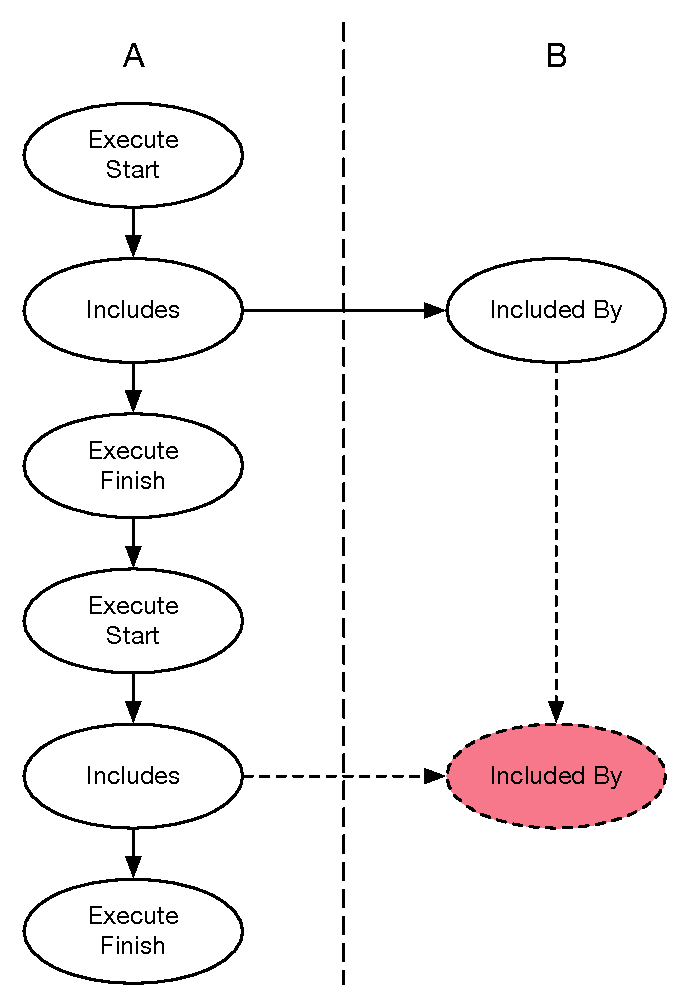
\includegraphics[width=\textwidth]{5validation/images/agreement-on-original-amount-of-executions-1.pdf}
			\caption{An example of two histories not agreeing on the amount of executions of A, violating \autoref{rule:agreement-on-the-original-amount-of-executions}.}
			\label{fig:agreement-on-the-original-amount-of-executions-1}
		\end{minipage}
		\hfill
		\begin{minipage}{.45\textwidth}
			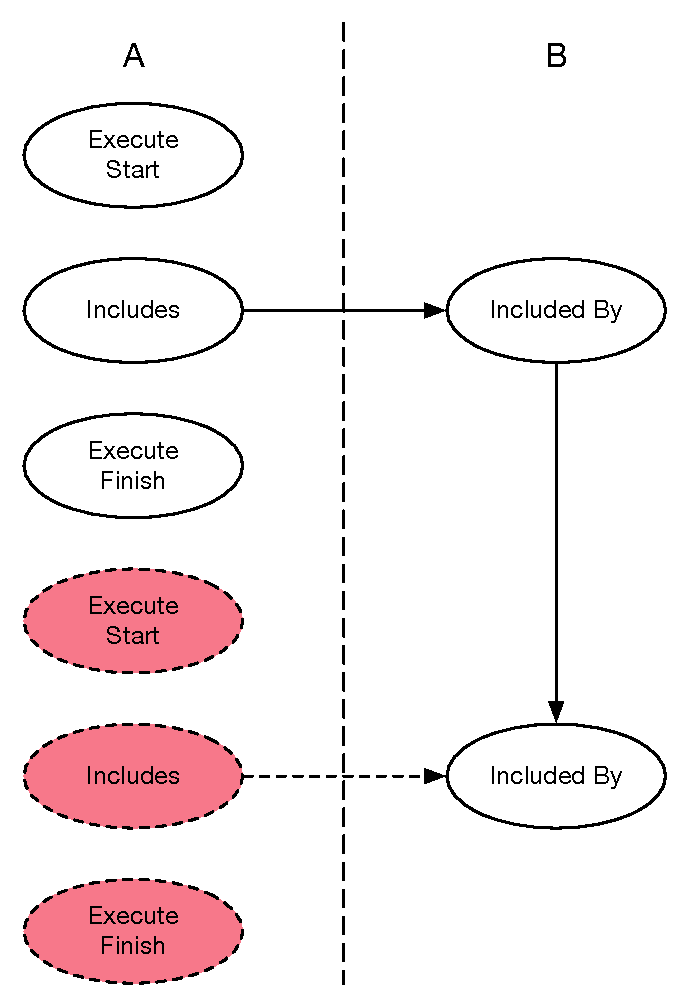
\includegraphics[width=\textwidth]{5validation/images/agreement-on-original-amount-of-executions-2.pdf}
			\caption{An example of two histories not agreeing on the amount of executions of A, violating \autoref{rule:agreement-on-the-original-amount-of-executions}.}
			\label{fig:agreement-on-the-original-amount-of-executions-2}
		\end{minipage}
	\end{figure}
	
	\newpar Recall that the definition of consistent cheating specified that actions could be added, removed or changed but the resulting history must still have the properties 2, 3 and 4 of valid histories. To argue that the rules \ref{rule:agreement-on-original-timestamps} and \ref{rule:agreement-on-the-original-amount-of-executions} cover the adding, removing and changing of actions each of these scenarios are examined:
	
	\begin{itemize}
		\item \textbf{Adding actions}: The rules of inconsistent cheating implies that the only consistent addition of actions are groups actions representing executions, or groups of actions representing the execution of other events affecting the current event. Rule  \ref{rule:agreement-on-the-original-amount-of-executions} handles this kind of violation.
		\item \textbf{Removing actions}: The rules of inconsistent cheating implies that the only consistent subtraction of actions are groups actions representing executions, or groups of actions representing the exection of other events affecting the current event. Rule  \ref{rule:agreement-on-the-original-amount-of-executions} handles this kind of violation.
		\item \textbf{Changing actions}: Recall that an action consists of an ID, a timestamp, a counterpart ID, a counterpart timestamp, and an action type. The rules of inconsistent cheating implies that it is not possible to change the ID, the counterpart ID, or the action type consistently. This leaves the timestamp and counterpart timestamp as the only two values which can be altered consistently, since unoriginal timestamp values can still abide to Lamport's logical clocks. Therefore \autoref{rule:agreement-on-original-timestamps} covers this violation.
	\end{itemize}
	
	\subsection{Detection Using DCR Graph Structure}
	Detecting and identifying consistently cheating processes is difficult, because it is not always possible to look at the history of a single event and determine if it is valid or not. It is now examined how the structure of the DCR graph and the placement of the malicious processes contribute to the ability to detect and identify consistent cheating. The type of relation has no influence on the cases and relations are therefore visualised as an arrow from event to event.
	
	\begin{case}
		In this case the workflow contains an event that does not share relations with any other event but may have relations to itself. If the event is hosted on a malicious process and it consistently cheats, there is no one to disagree with any timestamps on actions or oppose the amount of executions that have happened. Therefore in workflows with such a structure, it is not possible to identify or even observe if any kind of consistent cheating has happened on this event. 
		\label{case:malicious-alone}
	\end{case}
	
	\begin{case}
		In this case the workflow contains an event on a malicious process that has a relation to an event on a correct process as shown in \autoref{fig:consensus:single-malicious-with-good-relation}. The malicious process can cheat consistently with the timestamps in two ways: It can change the timestamps of the actions corresponding to the relations with the counterpart, but in that case the two events will not agree on what happened and it is observable that that one of the processes hosting the event must cheat. If the timestamp changes are on actions not related to the good event then it is not possible to observe nor identify. An example of this is has been shown on \autoref{fig:agreement-on-original-timestamps}.
		
		In the same way when looking at the amount of executions of the event on the malicious process, the malicious process might add more or remove some executions. In the case that it adds more executions, the event on the correct process will state that fewer executions happened, and vice versa. However the malicious process is not able to disagree with the number of executions of the event on the correct process consistently. 
		
		Therefore it is possible to observe but not identify consistent cheating in this case. 
		\label{case:malicious-to-good}
	\end{case}

	\begin{figure}[H]
		\centering
		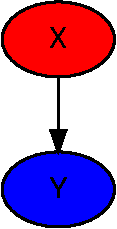
\includegraphics[]{5validation/images/3.pdf}
		\caption{A workflow containing an event on a malicious process that has a relation to an event on a correct process.}
		\label{fig:consensus:single-malicious-with-good-relation}
	\end{figure}
	
	\begin{case}
		In this case the workflow contains an event with a relation to an event on a malicious process as shown in \autoref{fig:consensus:single-good-with-malicious-relation}. Similarly to \autoref{case:malicious-to-good} timestamp changes are observable due to the same factors, but agreeing on exeuctions has another form. Instead of agreeing on the amount of executions of the event on the malicious process, the disagreement will be about the amount of executions of the event on the correct process. Furthermore the malicious process is free to report any number of executions as in case one because no event can disagree on any outgoing actions. 
		\label{case:good-to-malicious}
	\end{case}
	 
	\begin{figure}[H]
		\centering
		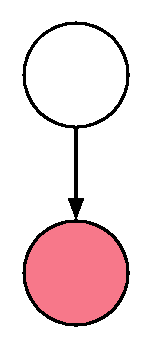
\includegraphics[]{5validation/images/2.pdf}
		\caption{A workflow containing an event on a correct process that has a relation to an event on a malicious process.}
		\label{fig:consensus:single-good-with-malicious-relation}
	\end{figure}

	\noindent Note that it is not possible to distinguish between disagreements as a result of cases \ref{case:malicious-to-good} and \ref{case:good-to-malicious}, since they can create the exact same histories with the exact same disagreements.
	
	\begin{case}
		In this case the workflow contains two events with relations to each other where one of the events is hosted on a malicious process, as shown on \autoref{fig:consensus:single-good-with-twoway-malicious-relation}. The ability to observe and identify consistent cheating is similar to that of the cases \ref{case:malicious-to-good} and \ref{case:good-to-malicious} because the two events are able to disagree on both timestamps and the amount of executions of both events.
	\end{case}
	
	\begin{figure}[H]
		\centering
		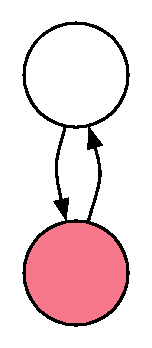
\includegraphics[]{5validation/images/6.pdf}
		\caption{A workflow containing an event on a malicious process and an event on a correct process where the events have relations to each other.}
		\label{fig:consensus:single-good-with-twoway-malicious-relation}
	\end{figure}
	
	\begin{case}
		In this case the workflow contains an event on a malicious process with a relation to another event on a malicious process as shown in \autoref{fig:consensus:single-malicious-with-twoway-malicious-relation}. The two processes can work in collaboration to manipulate the histories of the two events. 
		
		If it is assumed that they work in collaboration, then they are able to change timestamps and the amount of executions in such a way that it is not observable because it is present in both the histories. If they however do not change the timestamps or the amount of executions in collaboration, then they will disagree on the values and it is possible to observe that at least one of the processes are malicious.
		\label{case:malicious-to-malicious}
	\end{case}
	
	\begin{figure}[H]
		\centering
		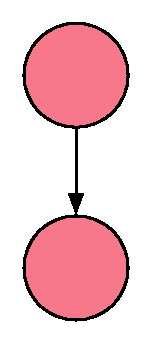
\includegraphics[]{5validation/images/4.pdf}
		\caption{A workflow containing two events on malicious processes where one event has a relation to the other.}
		\label{fig:consensus:single-malicious-with-twoway-malicious-relation}
	\end{figure}
	
	\begin{case}
		In this case the workflow contains two events hosted on malicious processes with relations to each other as shown in \autoref{fig:consensus:two-malicious-with-twoway-malicious-relation}. This situation has the same properties as \autoref{case:malicious-to-malicious}.
		\label{case:malicious-to-from-malicious}
	\end{case}

	\begin{figure}[H]
		\centering
		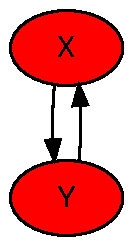
\includegraphics[]{5validation/images/7.pdf}
		\caption{A workflow containing two events on malicious processes where the events has relations to each other.}
		\label{fig:consensus:two-malicious-with-twoway-malicious-relation}
	\end{figure}
	
	\newpar It is not possible to identify which of the events are hosted on malicious processes, in any of these cases. Furthermore in cases \ref{case:malicious-alone}, \ref{case:malicious-to-malicious}, and \ref{case:malicious-to-from-malicious} it is not even possible to observe consistent cheating if the processes collaborate.
	
	\newpar This creates some interesting questions about how one can try to identify which of the events are cheating when cheating is observed. One method of doing so could be to determine the malicious process by counting how many of the neighbouring events disagree with the event on the process. If the majority of the neighbours disagree, the process hosting the event will be marked as malicious. Unfortunately that method has drawbacks since an event on a correct process with connections only to events on malicious processes could itself be marked as malicious. 
	
	If we require that in all neighbourhoods (the sets of neighbours of all events) of the DCR graph, with $N$ events, a maximum of $N/2-1$ events are hosted on malicious processes, then an election would not be able to falsely accuse an event on a correct process of being malicious. This requirement is often needed in distributed systems that use elections, but traditionally it is only used to describe the amount of malicious nodes in the entire system and not in each neighbourhood. Therefore this requirement is more strict and perhaps more difficult to accomplish.
	
	\newpar To make the situation substantially worse, even if this requirement is accomplished, a malicious process does not have to cheat with the actions related to a majority of neighbours of the event. An example could be a workflow with four events fully connected where one of the events is hosted on a malicious process. The malicious process could consistently cheat with one its relations but keep the rest of its history valid. In that situation only one of the neighbours would vote against it. 
	
	As described in the example it would be possible for the malicious process to trick an election into not having a majority against it. Therefore an election cannot conclude that a process \textit{is} correct, which leaves the situation no better than the initial situation, where it was only possible to detect that at least one of the processes were malicious.
	
	\newpar From the cases shown above it becomes apparent that the structure of the workflow has a great influence on whether or not it is possible to observe consistent cheating - especially in cases where a lot of malicious events are either interconnected or not connected to any other event at all. In these cases it can be difficult to observe any malicious activity. Furthermore, the cases also show that the more relations events on malicious processes have to events on correct processes and vice versa, the more it is possible to observe the malicious activity. Therefore a more connected workflow is preferred, because the probability for an event on a malicious process to be connected to an event on a correct process is higher.
	
%	\newpar One could argue the implications of consistent cheating in sub-graphs such as those of case 1 and 2, since their these events have little consequences on the rest of the workflow state. Therefore these events can only exist in two states (before and after they are executed) and therefore not being able to handle these kinds of situations is not that big a flaw. The major problems are apparent in situation 6 and 7 where, for example, a company can own a sub-part of the graph with many events working together to create a falsified image of what has actually happened. 


	\begin{table}[]
		\centering
		\label{table:inconsistent-cheating-properties}
		\begin{tabular}{lll}
			\textbf{Inconsistent Cheating} & \textbf{Observable} & \textbf{Identifiable} \\
			\textit{Rule 1 (Only specified relations)}         & Yes          & No            \\
			\textit{Rule 2 (Only complete executions)}         & Yes          & No            \\
			\textit{Rule 3 (Executions only in valid states)}  & Yes          & No            \\
			\textit{Rule 4 (Only non disrupted executions)}    & Yes          & Yes            \\
			\textit{Rule 5 (Wait for complete execution)}      & Yes          & Yes            \\
			\textit{Rule 6 (Synchronous message exchange)}     & Yes          & Yes            \\
			\textit{Rule 7 (Total order of timestamps)}        & Yes        & Yes            \\
			\textit{Rule 8 (Message exchange timestamp order)} & Yes          & Yes           
		\end{tabular}
		\caption{Table of the observability and identifiability of the different inconsistent cheating types}
	\end{table}
	
	\begin{table}[]
		\centering
		\label{my-label}
		\begin{tabular}{llll}
			\textbf{Consistent Cheating} & \textbf{Agreement on original timestamps} & \textbf{Agreement on amount of executions (incoming)} & \textbf{Agreement on amount of executions (outgoing)} \\
			\textit{Case 1}              & Not observable                   & Not observable                               & Not observable                               \\
			\textit{Case 2}              & Not observable                   & Not observable                               & Not observable                               \\
			\textit{Case 3}              & Not observable                   & Not observable                               & Not observable                               \\
			\textit{Case 4}              & Not observable                   & Not observable                               & Not observable                               \\
			\textit{Case 5}              & Not observable                   & Not observable                               & Not observable                               \\
			\textit{Case 6}              & Not observable                   & Not observable                               & Not observable                              
		\end{tabular}
		\caption{There should be a caption here.}
	\end{table}
	\todo{write about it}

    \section{Simulation}\label{sec:historyindcr:simulation}
    One of the more difficult validity properties to check is whether events have executed only when the state of the workflow allowed it. To do so, a lot of challenges must be addressed, it is not enough to check if the initial state of the event is executable, its conditions also need to be taken into perspective, furthermore the state of the workflow most likely changes over time with each execution. In addition since the history is a strictly partially ordered set, some executions happen concurrently which does not match physical time in which the events have executed.\todo[inline]{Jeg har lidt svært ved at indlede dette afsnit, men jeg synes ikke det skal starte med at det her er sværere end de andre validations.}
    
    \newpar One approach to this problem is to simulate the executions of the workflow. To do so, it is required that the rules of the workflow and the initial state of every event in the workflow is known. Furthermore it is required that an order of execution has been found, this is examined in the next chapter but we assume it is available. 
    
    Given the order of execution each execution has either zero or more ingoing edges. Each ingoing edge states which executions must have happened before, therefore an execution can first happen when all of its ingoing edges have executed. Therefore each execution have a counter based on the amount of ingoing edges which can be decreased each time one of the ingoing edges executes. An order of execution based on a valid history will always have some executions which have no ingoing edges since no cycles appear and some events \todo{executions? eller?}must happen before all their relations.
    
    \newpar To check if the execution of an event is possible, it is checked if the event is included and that the state of every condition of the event is either excluded or executed.\todo[inline]{Behøver vi skrive hvad det vil sige at være executable?} If the event was executable, the state of the workflow is changed according to the rules of the workflow.\todo[inline]{Vi opdaterer også state selvom den ikke er executable}
    
    \newpar To simulate the entire order of execution, the executions are checked for their ability to execute in a topological order. One way to create a topological order from an order of execution is to map each of the executions to the amount of executions that happens directly before an execution itself. An execution can be chosen as the next if and only if its counter reaches 0. When an execution is chosen, all of the executions it happens before has their counter decremented by 1. The order of which executions have happened are adhered to, but concurrent executions happen in a random order.\todo[inline]{Mikael: Jeg har omskrevet det her lidt, men ladet nogle sætninger være. Check gerne at det giver mening}
    
    Executions can only be concurrent if the events they belong to do not share outgoing relations. If two events share outgoing relations, one of them must affect the shared event before the other and an order would be able to be created. Therefore in an order of execution only one of the ingoing edges can be of an ingoing relation, the rest must be based on outgoing relations which can determine that the execution happens after some other execution. The order of which concurrent executions are simulated therefore does not matter since they order of which they execute can only result in one state change which affects common outgoing edges.\todo[inline]{hvad siger vi her?}
    
    \newpar If an execution was not executable, it is possible to identify if it is the event itself which is malicious or if it is one or more of the condition events. If the state of the event was not executable then the event must be malicious, note that the conditions in this case also could be malicious. If the state is executable and the conditions are included and not executed, another situation arises. The conditions could have returned false information to the executing event, or the executing event could have executed regardless of the values returned. Therefore in this case only a set of possible malicious events can be determined.\todo[inline]{Mikael: Jeg har svært ved at forstå hvad vi vil med denne paragraf. Måske en figur kan hjælpe?}
    \todo[inline]{Fisk: Jeg har generelt at forstå det her afsnit. Det skal vi nok lige gå igennem igen.}

	\newpar In \autoref{alg:simulation} the simulation algorithm can be seen. It runs in time linear to the amount of executions.
	
	\figuretodo{figur over en order of executions med counters på hver executions - eventuelt en ekstra med hvordan det ser ud efter at x events har executed. Mikael: For mig er det ikke det essentielle ved algoritmen "Simulation".}
	
	\begin{algorithm}[H]
		\begin{algorithmic}
			\Function{Simulation}{orderOfExecution, DCRRules, state}
			\State orderedExecutions $\leftarrow$ \Call{TopilogicalSort}{orderOfExecution} \Comment Returns a queue
			\State failures $\leftarrow$ List.Empty
			\While{not orderedExecutions.isEmpty}
				\State execution $\leftarrow$ \Call{Queue.Pop}{orderedExecutions}
					\If{not \Call{IsExecutable}{execution.Event, state}}
					\State failures $\leftarrow$ \Call{List.Add}{execution, failures}
				\EndIf
				\State state $\leftarrow$ \Call{ApplyExecution}{execution.Event, DCRRules, state}
			\EndWhile
			\State\Return failures
			\EndFunction
		\end{algorithmic}
		\caption{The \textbf{Simulation} algorithm}
		\label{alg:simulation}
	\end{algorithm}
	\todo[inline]{Check lige op på algoritmen generelt}
	
	\newpar This algorithm is based on the forward chaining algorithm of entailment in propositional theorem proving\todo{ref section 7.5 in SISP bog. Mikael: Jeg synes det er fedt at vi har anvendt viden fra det fag, men synes at det stikker lidt uden for de ting vi har sagt er nødvendigt for at forstå denne opgave. Jeg har også forsøgt at formulere i teksten ovenfor hvordan man kan anvende algoritmen til at finde denne order, men uden at gå alt for teknisk til værks.}, which also runs in linear time and is used to see if a knowledge base can entail a proposition.
	
    \newpar There is a couple of challenges and approaches to how it is handled both if cheating has been observed before the simulation or cheating is observed during the simulation. We have chosen the approach to mark if an execution was inconsistent, but allow it to "execute" and then change the state to see if the rest of the order of execution was consistent. One could easily check the rest of the order of execution without the state change of the inconsistent execution to see what implications that cheating could have had.
    
    \todo[inline]{Flyttet fra Background herfra...}
    The reason why typical Byzantine general problem algorithms cannot be used in this project is that the commander needs to use information from the potentially malicious processes to decide on a correct value to propose. Again since at most two events share the information the requirement that maximum $f=N/3$ malicious is not kept in regards to information gathering and it is therefore impossible to get ensure correct information from each event.\todo{måske er der noget af det her der skal rykkes ned i validation og election så vi faktisk bare beskriver hvad det er.}
    Furthermore, most consensus algorithms require all processes of the election to be able to propose a value which should be agreed upon, but since each DCR event does not know nor is able to produce the entire history of the workflow, and therefore cannot propose a value which other events would be able to agree on, such algorithms cannot be used.\todo[inline]{... Flyttet fra Background hertil}
    
    \section{Observability and identifiability}
    
    \section{Correctness}
    Note that property 1 must be violated in order to violate either property 2, 3, or 4. 
    
    If it is possible to detect both consistent and inconsistent cheating, then it is possible to decide if a history is valid or invalid.